\subsubsection{Analisi dei requisiti}
\paragraph{Scopo}\mbox{}\\ \\
L'analisi dei requisiti è un'attività che avviene prima di quella di sviluppo.\\
Il documento \AdR{}, redatto dagli analisti, ha come scopo i seguenti punti:
\begin{itemize}
\item Definire lo scopo del prodotto da realizzare;
\item Fissare le funzionalità del progetto concordate col proponente;
\item Fornire ai progettisti riferimenti precisi ed affidabili per la progettazione dell'architettura software;
\item Definire una base per integrare i raffinamenti che permettono un miglioramento continuo del prodotto e del \glo{processo} di sviluppo;
\item Fornire ai verificatori dei riferimenti per l’attività di controllo;
\item Fornire una stima del quantitativo di lavoro da svolgere per tracciare una stima dei costi. 
\end{itemize}

\paragraph{Aspettative}\mbox{}\\ \\
L'obiettivo è quello di creare un documento formale contenente tutti i \glo{requisiti} richiesti e concordati col proponente.
Deve essere possibile fare riferimento a quanto redatto nel documento \AdR{} qualora sorgessero incomprensioni e dubbi al momento del collaudo del prodotto.

\paragraph{Casi d'uso}\mbox{}\\ \\
Definiscono uno scenario in cui uno o più attori interagiscono con il sistema.
\subparagraph*{Codice identificativo dei casi d'uso}\mbox{}\\
Il codice identificativo di ciascun caso d’uso, univoco nel suo complesso, segue la sintassi qui indicata:
\begin{center}
	\textbf{UC[Destinazione] [Codice]}
\end{center}
con:
\begin{itemize}
	\item \textbf{[Destinazione]}:
		\begin{itemize}
			\item \textbf{A}, se il caso d’uso descrive un comportamento o una funzione che l’\glo{utente} ha a disposizione nell'applicazione mobile;
			\item \textbf{S}, se il caso d’uso descrive un comportamento o una funzione che l'\glo{amministratore} ha a disposizione nell'applicazione web.
		\end{itemize}
	\item \textbf{[Codice]} (dati X, Y, Z $\in \mathbb{Z_+}$):
	\begin{itemize}
		\item \textbf{X}, se il caso d'uso è di tipo \glo{kite-level};
		\item \textbf{X.Y}, se il caso d'uso è di tipo \glo{sea-level};
		\item \textbf{X.Y.Z}, se il caso d'uso è di tipo \glo{fish-level}.
	\end{itemize}
\end{itemize}

\subparagraph*{Struttura di un caso d'uso kite-level}\mbox{}\\ \\
La seguente è una struttura ad elenco che un caso d'uso \glo{kite-level} necessariamente deve adottare.\\
I punti dell'elenco racchiusi fra parentesi quadre (non sono inclusi fra questi [Destinazione] e [Codice]) indicano che tale punto è opzionale e va inserito solo se necessario.\\
\textbf{UC[Destinazione] X - Nome del caso d'uso kite-level. Stile tipografico: lettera maiuscola iniziale per ciascun attore, attori separati da virgola, nessun punto fermo alla fine.} %kite level
\begin{itemize}
	\item \textbf{Attori primari}: Elenco degli attori primari.
	Stile tipografico: lettera maiuscola iniziale per ciascun attore, attori separati da virgola, nessun punto fermo alla fine.
	\item \textbf{[Attori secondari}: Elenco degli attori secondari.
	Stile tipografico: lettera maiuscola iniziale per ciascun attore, attori separati da virgola, nessun punto fermo alla fine.]
	\item \textbf{Precondizione}: Stato in cui si trova il sistema prima dell'esecuzione del caso d'uso.
	Stile tipografico: lettera maiuscola a inizio frase, punto fermo alla fine.
	\item \textbf{Postcondizione}: Stato in cui si trova il sistema dopo l'esecuzione del caso d'uso.
	Se l'attore è cambiato alla fine dell'esecuzione, va indicato.
	Stile tipografico: lettera maiuscola a inizio frase, punto fermo alla fine.
	\item \textbf{Scenario principale}: Descrizione testuale, non un elenco puntato, di quello che avviene durante l'esecuzione del caso d'uso, ovvero cosa succede affinché date le precondizioni si ottengano le postcondizioni.
	Stile tipografico: lettera maiuscola a inizio frase, punto fermo alla fine.
	\item \textbf{[Scenario alternativo}: Descrizione testuale, non un elenco puntato, di quello che può avvenire durante l'esecuzione del caso d'uso che si discosta dalla sua normale esecuzione (ad esempio un'anomalia), ovvero cosa succede affinché date le precondizioni non si ottengano le postcondizioni.
	Stile tipografico: lettera maiuscola iniziale per ciascun attore, attori separati da virgola, nessun punto fermo alla fine.
	Nota: se ci sono più scenari alternativi, marcare il primo come \textbf{Scenario alternativo 1} e proseguire ordinatamente con \textbf{Scenario alternativo 2}, ecc.]
	\item \textbf{[Flusso di eventi}: Elenco ordinato di eventi che accadono e permettono il raggiungimento  della postcondizione.
	Stile tipografico: gli elementi intermedi dell'elenco terminano con un punto e virgola, mentre l'ultimo con un punto fermo.]
	\item \textbf{[Generalizzazione}: Caso d'uso che è generalizzazione del caso d'uso in esame.]
	\item \textbf{[Inclusioni}: Elenco non ordinato dei casi d'uso (\textbf{UC[Destinazione] [Codice] - Nome del caso d'uso}) che permettono di raggiungere le postcondizioni indicate.
	Tipicamente si ottengono inclusioni da casi d'uso di tipo \glo{sea-level}, \glo{fish-level}.
	Il caso d'uso descritto non conosce i dettagli dei casi d'uso inclusi ma solo i loro risultati.
	Questi casi d'uso non sanno di essere inclusi e la loro esecuzione dipende completamente dal caso d'uso che si sta descrivendo.
	Stile tipografico: gli elementi intermedi dell'elenco terminano con un punto e virgola, mentre l'ultimo con un punto fermo.]
	\item \textbf{[Estensioni}: Elenco non ordinato dei casi d'uso (\textbf{UC[Destinazione] [Codice] - Nome del caso d'uso}) che estendono la normale esecuzione del caso d'uso che si sta descrivendo, deviandola e impedendo il raggiungimento delle postcondizioni.
	Tipicamente è un elenco di casi d'uso \glo{sea-level} o \glo{fish-level}.
	Stile tipografico: gli elementi intermedi dell'elenco terminano con un punto e virgola, mentre l'ultimo con un punto fermo.]
\end{itemize}

\subparagraph*{Struttura di un caso d'uso sea-level}\mbox{}\\ \\
La seguente è una struttura ad elenco che un caso d'uso \glo{sea-level} necessariamente deve adottare.\\
I punti dell'elenco racchiusi fra parentesi quadre (non sono inclusi fra questi [Destinazione] e [Codice]) indicano che tale punto è opzionale e va inserito solo se necessario.\\
\textbf{UC[Destinazione] X.Y - Nome del caso d'uso sea-level. Stile tipografico: lettera maiuscola iniziale per ciascun attore, attori separati da virgola, nessun punto fermo alla fine.}%sea level
\begin{itemize}
	\item \textbf{Attori primari}: Come in UC[Destinazione] X.
	\item \textbf{[Attori secondari}: Come in UC[Destinazione] X.]
	\item \textbf{Precondizione}: Come in UC[Destinazione] X.
	\item \textbf{Postcondizione}: Come in UC[Destinazione] X.
	\item \textbf{Scenario principale}: Come in UC[Destinazione] X.
	\item \textbf{[Scenario alternativo}: Come in UC[Destinazione] X.]
	\item \textbf{[Flusso di eventi}: Come in UC[Destinazione] X.]
	\item \textbf{[Generalizzazione}: Come in UC[Destinazione] X.]
	\item \textbf{[Inclusioni}: Elenco non ordinato dei casi d'uso (\textbf{UC[Destinazione] [Codice] - Nome del caso d'uso}) che permettono di raggiungere le postcondizioni indicate.
	Tipicamente si ottengono inclusioni da casi d'uso di tipo \glo{fish-level}.
	Il caso d'uso descritto non conosce i dettagli dei casi d'uso inclusi ma solo i loro risultati.
	Questi casi d'uso non sanno di essere inclusi e la loro esecuzione dipende completamente dal caso d'uso che si sta descrivendo.
	Stile tipografico: gli elementi intermedi dell'elenco terminano con un punto e virgola, mentre l'ultimo con un punto fermo.]
	\item \textbf{[Estensioni}: Elenco non ordinato dei casi d'uso (\textbf{UC[Destinazione] [Codice] - Nome del caso d'uso}) che estendono la normale esecuzione del caso d'uso che si sta descrivendo, deviandola e impedendo il raggiungimento delle postcondizioni.
	Tipicamente è un elenco di casi d'uso \glo{fish-level}.
	Stile tipografico: gli elementi intermedi dell'elenco terminano con un punto e virgola, mentre l'ultimo con un punto fermo.]
\end{itemize}

\subparagraph*{Struttura di un caso d'uso fish-level}\mbox{}\\ \\
La seguente è una struttura ad elenco che un caso d'uso \glo{fish-level} necessariamente deve adottare.\\
I punti dell'elenco racchiusi fra parentesi quadre (non sono inclusi fra questi [Destinazione] e [Codice]) indicano che tale punto è opzionale e va inserito solo se necessario.\\
\textbf{UC[Destinazione] X.Y.Z - Nome del caso d'uso fish-level. Stile tipografico: lettera maiuscola iniziale per ciascun attore, attori separati da virgola, nessun punto fermo alla fine.}%sea level
\begin{itemize}
	\item \textbf{Attori primari}: Come in UC[Destinazione] X.
	\item \textbf{[Attori secondari}: Come in UC[Destinazione] X.]
	\item \textbf{Precondizione}: Come in UC[Destinazione] X.
	\item \textbf{Postcondizione}: Come in UC[Destinazione] X.
	\item \textbf{Scenario principale}: Come in UC[Destinazione] X.
	\item \textbf{[Flusso di eventi}: Come in UC[Destinazione] X.]
	\item \textbf{[Generalizzazione}: Come in UC[Destinazione] X.]
	\item \textbf{[Inclusioni}: Come in UC[Destinazione] X.]
	\item \textbf{[Estensioni}: Come in UC[Destinazione] X.]
\end{itemize}

\paragraph{Template di diagramma di caso d'uso}\mbox{}\\ \\
Il seguente è un esempio di diagramma di caso d'uso con tutte le possibili componenti \glo{UML} da usare per realizzare i diagrammi dei casi d'uso.
\begin{figure}[h]
	\centering	
	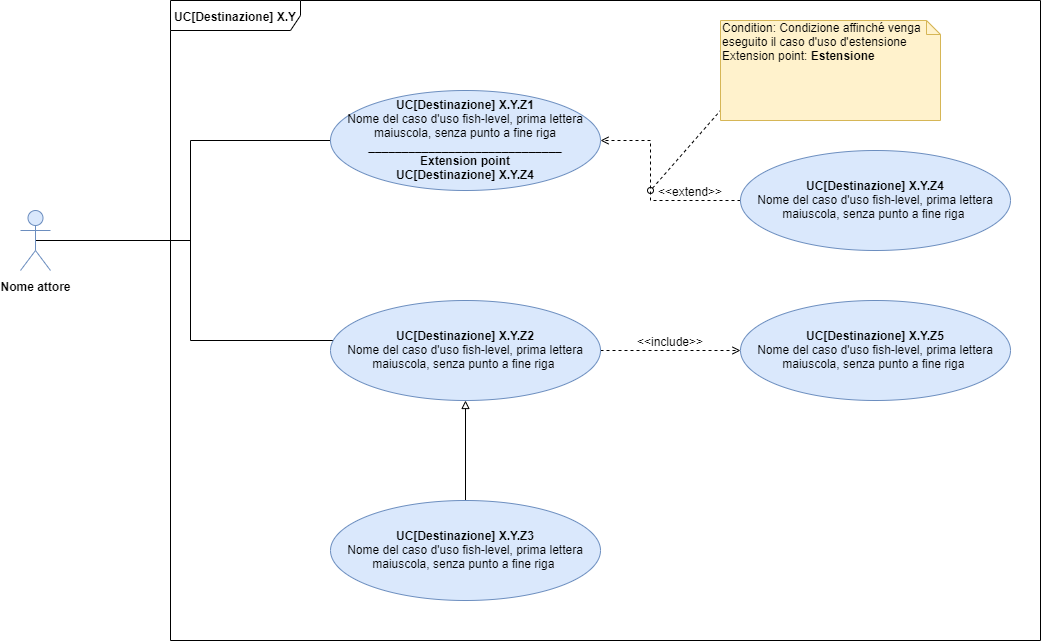
\includegraphics[scale=0.45]{Immagini/TemplateSchemaUseCase.png}
	\caption{UC[Destinazione] X.Y - Template di diagramma di caso d'uso}
\end{figure}

\paragraph{Casi d'uso d'errore e dei messaggi informativi}\mbox{}\\ \\
L'ultimo caso d'uso \glo{kite-level}, sia lato applicazione (\textbf{UCA}) che lato server (\textbf{UCS}), contiene tutti i casi d'uso che descrivono situazioni d'errore e situazioni in cui l'attore del caso d'uso deve essere informato con un messaggio per tutti i casi d'uso lato applicazione e lato server rispettivamente.\\
\'E stato scelto di raggruppare i casi d'uso degli errori in questa maniera per favorirne il riuso.
% Questa decisione viene presa per avere un unico punto in cui concentrare tutte queste situazioni.
\paragraph{Requisiti}\mbox{}\\ \\
Un requisito è un obiettivo da raggiungere per risolvere un problema, necessario per almeno uno stakeholder o una caratteristica che deve essere soddisfatta per esaudire una richiesta di uno stakeholder. \\
I requisiti vengono organizzati in forma tabellare, che deve contenere le seguenti colonne:
\begin{itemize}
	\item Codice identificativo di un requisito;
	\item Classificazione;
	\item Descrizione;
	\item Fonti.
\end{itemize}

\subparagraph*{Codice identificativo dei requisiti}\mbox{}\\ \\
Il codice identificativo di ciascun requisito, univoco nel suo complesso, segue la sintassi qui indicata:
\begin{center}
	\textbf{R[Importanza][Tipologia][Codice]}
\end{center}
con:
\begin{itemize}
	\item \textbf{[Importanza]}:
	\begin{itemize}
		\item \textbf{1}: Requisito obbligatorio, ovvero irrinunciabile per almeno uno degli stakeholder;
		\item \textbf{2}: Requisito desiderabile, ovvero non strettamente necessario ma che porta valore aggiunto riconoscibile;
		\item \textbf{3}: Requisito opzionale, ovvero relativamente utile oppure contrattabile più avanti nel progetto.
	\end{itemize}
	\item \textbf{[Tipologia]}:
	\begin{itemize}
		\item \textbf{F}: Funzionale, definisce una funzione di uno o più componenti del sistema;
		\item \textbf{Q}: Qualitativo, definisce un requisito per garantire la qualità per un determinato aspetto del prodotto;
		\item \textbf{P}: Prestazionale, definisce un requisito che garantisce efficienza prestazionale nel prodotto;
		\item \textbf{V}: Vincolo, definisce un requisito volto a far rispettare un dato vincolo presente nel capitolato.
	\end{itemize}
	\item \textbf{[Codice]}:
	\begin{itemize}
		\item A*\ap{1} se il requisito proviene da un caso d'uso dell'applicazione, dove al posto di *\ap{1} è presente: il valore X (numero del caso d'uso kite-level) del codice identificativo del caso d'uso, seguito da un punto e un numero progressivo;
		\item S*\ap{2} se il requisito proviene da un caso d'uso del server, dove al posto di *\ap{2} è presente: il valore X (numero del caso d'uso kite-level) del codice identificativo del caso d'uso, seguito da un punto e un numero progressivo;
		\item C*\ap{3} se il requisito proviene dal capitolato, dove al posto di *\ap{3} è presente un numero progressivo;
		\item V*\ap{4} se il requisito proviene da un verbale, dove al posto di *\ap{4} è presente: il numero che indica il verbale da cui proviene il requisito; il numero si calcola a partire da 1, che sarà associato al primo verbale redatto (in ordine temporale). Infine vi sarà un punto seguito dal numero progressivo;
		\item I*\ap{5} se il requisito proviene da una decisione presa internamente al gruppo, dove al posto di *\ap{5} è presente: un numero progressivo.
	\end{itemize}
\end{itemize}

\subparagraph*{Struttura di un requisito}\mbox{}\\ \\
La seguente è una descrizione di una riga della tabella in cui vengono elencati i \glo{requisiti}.

{
\rowcolors{2}{grigetto}{white}
\renewcommand{\arraystretch}{1.5}
\centering
\begin{longtable}{C{3cm} C{3.2cm} C{4.3cm} C{4.3cm}}
\rowcolor{darkblue}
\textcolor{white}{\textbf{Identificativo}} &
\textcolor{white}{\textbf{Descrizione}} &
\textcolor{white}{\textbf{Classificazione}} &
\textcolor{white}{\textbf{Fonti}} \\
\endhead
Codice identificativo del requisito &
Descrizione sintetica, ma al contempo esaustiva, del requisito &
Informazione ridondante, sotto forma testuale, dell’importanza del requisito. Facilita la lettura dei requisiti &
Definisce da dove deriva il requisito. I requisiti vengono raccolti da una o più fonti tra quelle citate di seguito:
\begin{itemize}
	\item Capitolato;
	\item Interno (ritenuto opportuno dagli analisti);
	\item Casi d'uso (riportare i codici identificativi);
	\item Verbale (riportare il codice identificativo).
\end{itemize} \\
\end{longtable}
}